\documentclass[tikz,border=10pt]{standalone}
\usepackage{tikz}
\usepackage{makecell}

\usetikzlibrary{arrows}
\usetikzlibrary{circuits.logic.US}
\usetikzlibrary{matrix}
\usetikzlibrary{positioning}
\usetikzlibrary{backgrounds}
\usetikzlibrary{decorations.pathreplacing, positioning, shapes.geometric, shapes.misc, shadows, fit}
\usetikzlibrary{shapes.geometric, shapes.symbols, arrows, shadows, fit, backgrounds, 3d, plotmarks, calc, intersections, matrix, patterns}

\tikzstyle{thin_arrow} = [draw,->,>=stealth]
\tikzstyle{arrow} = [thick,thin_arrow]
\tikzstyle{bidir_arrow} = [draw,thick,<->,>=stealth]
\tikzstyle{graph_node} = [draw, circle, inner sep=0.5pt, font=\footnotesize]
\tikzstyle{lb_color} =  [top color=cyan!5, bottom color=cyan!15]
\tikzstyle{lb} =  [rectangle, anchor=south west, draw, lb_color]
\tikzstyle{large_lb} = [lb, minimum width=1.5cm, minimum height=1.5cm]
\tikzstyle{ram} = [rectangle, anchor=south west, draw, top color=teal!10, bottom color=teal!20]
\tikzstyle{dsp} = [rectangle, anchor=south west, draw, top color=olive!30, bottom color=olive!40]

\tikzstyle{trapezoid} = [trapezium,
                    trapezium stretches=true,
                    trapezium left angle=70,
                    trapezium right angle=110,
                    ]

\tikzstyle{io} = [trapezoid,
                    minimum width=2.5cm,
                    minimum height=1cm,
                    text centered,
                    align=center,
                    draw=black,
                    drop shadow,
                    top color=blue!10,
                    bottom color=blue!30]

\tikzstyle{design} = [io]
\tikzstyle{metric} = [io,
                      minimum width=1cm]

\tikzstyle{device} = [rounded rectangle,
                    minimum width=3cm,
                    minimum height=1cm,
                    text centered,
                    align=center,
                    draw=black,
                    drop shadow,
                    top color=black!10!green!20,
                    bottom color=black!10!green!70]

\tikzstyle{process} = [rectangle,
                        minimum width=3cm,
                        minimum height=1cm,
                        text centered,
                        align=center,
                        draw=black,
                        drop shadow,
                        top color=orange!10,
                        bottom color=orange!35]

\tikzstyle{process_no_shadow} = [rectangle,
                        minimum width=3cm,
                        minimum height=1cm,
                        text centered,
                        align=center,
                        draw=black,
                        top color=orange!10,
                        bottom color=orange!35]

\begin{document} 

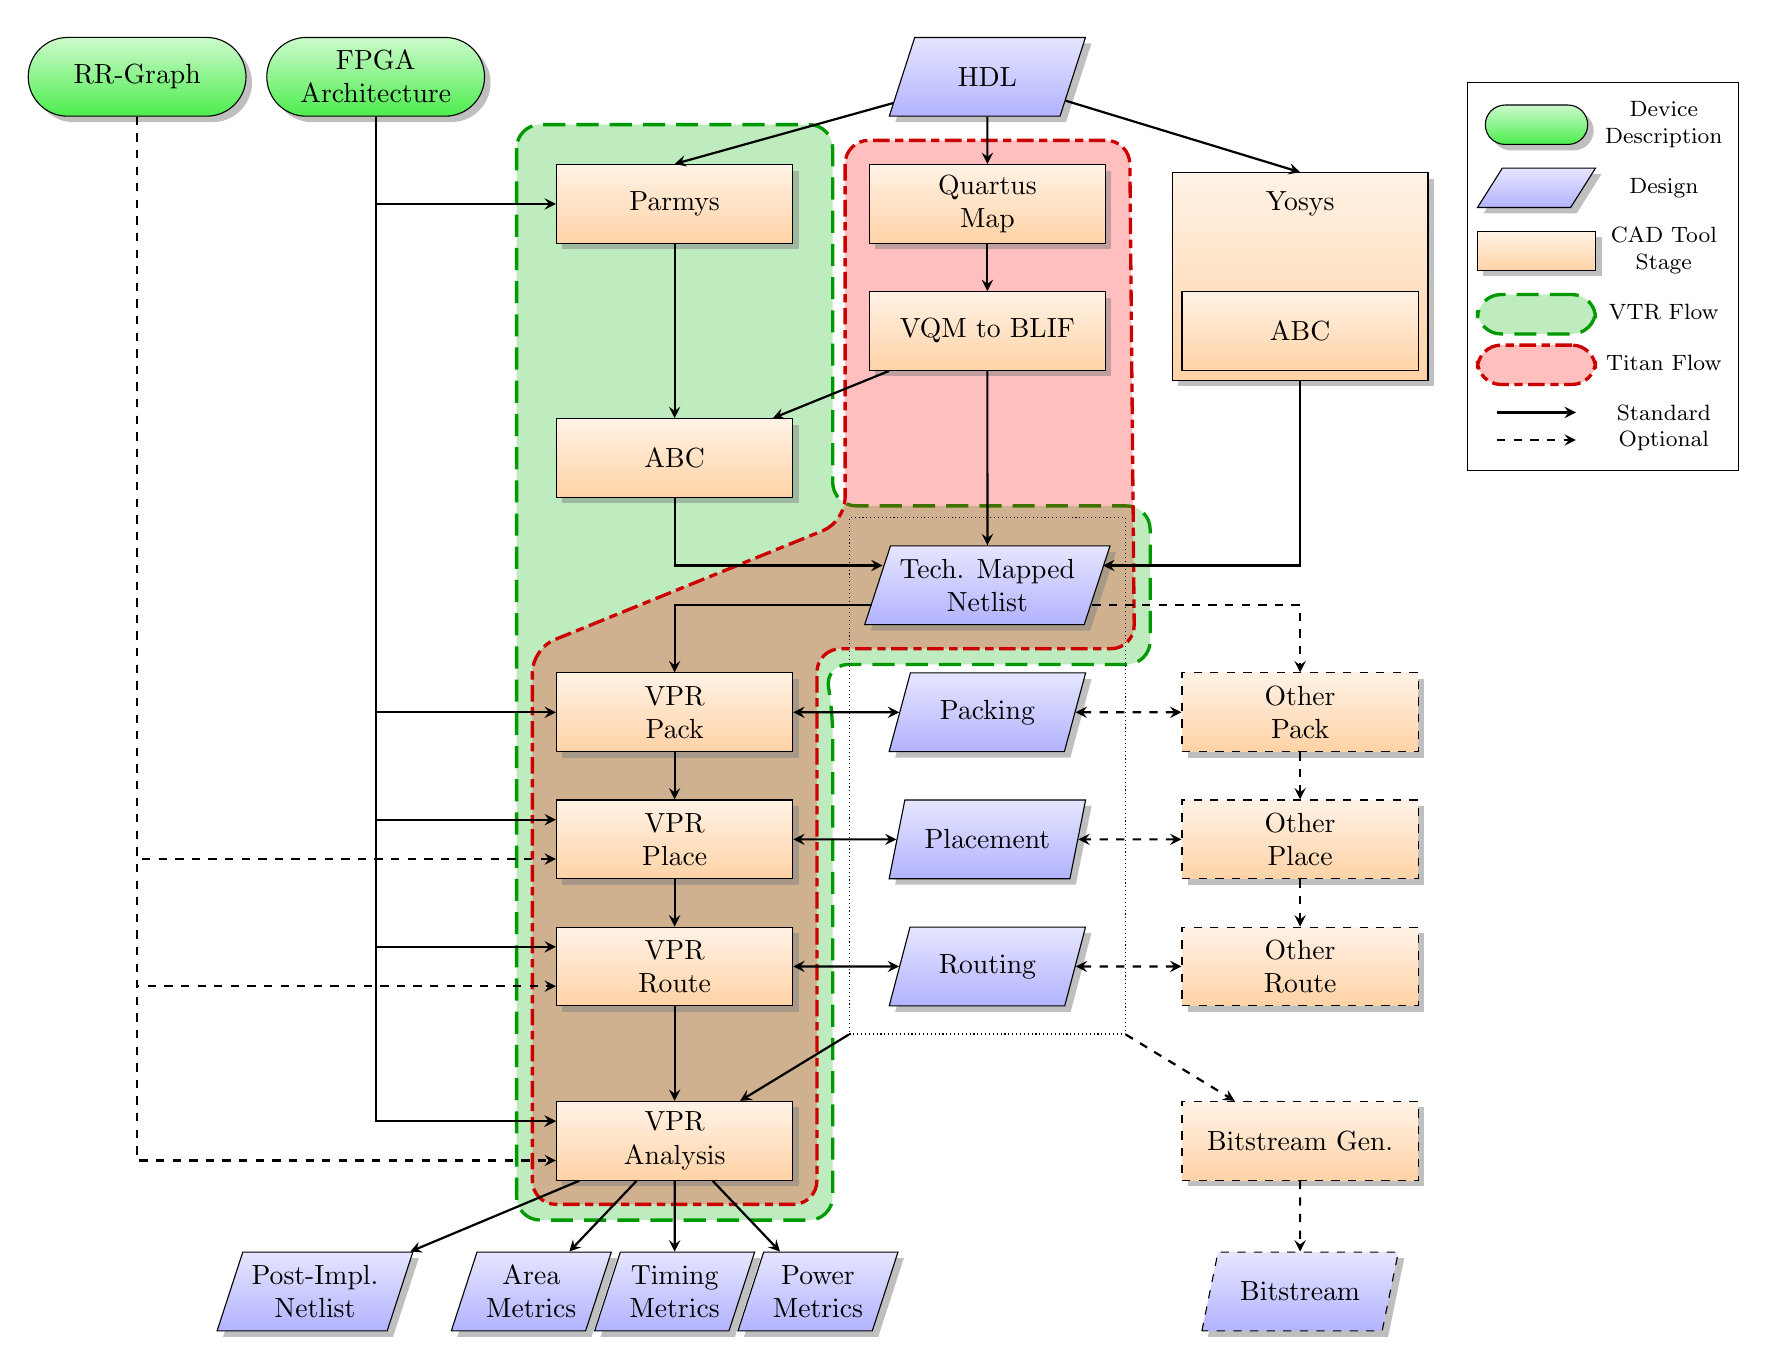
\begin{tikzpicture}[node distance=1.0cm]
    \tikzstyle{vtr_callout} = [draw=black!40!green, fill=black!30!green, fill opacity=0.25, very thick, dash pattern={on 8pt off 4pt}, rounded corners=0.3cm]
    \tikzstyle{titan_callout} = [draw=black!20!red, fill=red, very thick, fill opacity=0.25, dash pattern={on 6pt off 2pt on 3pt off 2pt}, rounded corners=0.3cm]

    \pgfmathsetmacro{\vtroffset}{0.5cm}
    \pgfmathsetmacro{\titanoffset}{0.3cm}
    \pgfmathsetmacro{\metricoffset}{0.6cm}

    \newcommand{\arrowshift}{0.25cm}
    \newcommand{\arrowxshift}{0.07cm}

    \matrix [row sep=0.6cm, column sep=0.9cm] {
        \node (arch) [device] {FPGA \\ Architecture}; & & \node (hdl) [design] {HDL}; & \\
        & \node (parmys_synth) [process] {Parmys}; & \node (quartus_map) [process] {Quartus \\ Map}; & \node (yosys_frontend) [] {Yosys}; \\
        & & \node (vqm2blif) [process] {VQM to BLIF}; & \node (abc_yosys) [process_no_shadow] {ABC}; \\
        & \node (abc_synth) [process] {ABC}; & & \\
        & & \node (techmapped_netlist) [design] {Tech. Mapped \\ Netlist}; & & \\
        & \node (vpr_pack) [process] {VPR \\ Pack}; & \node (packing) [design] {Packing}; & \node (other_pack) [process, dashed] {Other \\ Pack}; & \\
        & \node (vpr_place) [process] {VPR \\ Place}; & \node (placement) [design] {Placement}; & \node (other_place) [process, dashed] {Other \\ Place}; & \\
        & \node (vpr_route) [process] {VPR \\ Route}; & \node (routing) [design] {Routing}; & \node (other_route) [process, dashed] {Other \\ Route}; & \\
        & & & & \\
        & \node (vpr_analysis) [process] {VPR \\ Analysis}; & & \node (assembler) [process, dashed] {Bitstream Gen.}; & \\
    };
    \node(rr_graph) [device,left=0.25cm of arch] {RR-Graph}; 

    \begin{scope}[on background layer]
        \node (yosys) [process, fit=(yosys_frontend) (abc_yosys)] {};
    \end{scope}

    \node (implementation) [draw, densely dotted, inner sep=0.35cm, fit=(techmapped_netlist) (packing) (placement) (routing)] {};

    \node (bitstream) [design, below=0.9cm of assembler, dashed] {Bitstream};

    \node (timing) [metric, below=0.9cm of vpr_analysis] {Timing \\ Metrics};
    \node (area) [metric, left=0.1cm of timing] {Area \\ Metrics};
    \node (power) [metric, right=0.1cm of timing] {Power \\ Metrics};
    \node (post_impl_netlist) [design, left=0.8cm of area] {Post-Impl. \\ Netlist};

    \draw [arrow] (arch) |- (parmys_synth);
    \draw [arrow] (arch) |- (vpr_pack.west);
    \draw [arrow] (arch) |- ([yshift=\arrowshift]vpr_place.west);
    \draw [arrow] (arch) |- ([yshift=\arrowshift]vpr_route.west);
    \draw [arrow] (arch) |- ([yshift=\arrowshift]vpr_analysis.west);
    \draw [arrow] (arch) |- ([yshift=\arrowshift]vpr_analysis.west);

    \draw [arrow] (hdl) -- (parmys_synth.north);
    \draw [arrow] (hdl) -- (quartus_map);
    \draw [arrow] (hdl) -- (yosys.north);
    \draw[arrow] (parmys_synth) -- (abc_synth);
    \draw[arrow] (quartus_map) -- (vqm2blif);
    \draw[arrow] (yosys) |- ([yshift=\arrowshift,xshift=\arrowxshift]techmapped_netlist.east);
    \draw[arrow] (vqm2blif) -- (abc_synth);
    \draw[arrow] (vqm2blif) -- (techmapped_netlist);
    \draw[arrow] (abc_synth) |- ([yshift=\arrowshift,xshift=\arrowxshift]techmapped_netlist.west);

    \draw[arrow] ([yshift=-\arrowshift,xshift=-\arrowxshift]techmapped_netlist.west) -| (vpr_pack);
    \draw[arrow, dashed] ([yshift=-\arrowshift,xshift=-\arrowxshift]techmapped_netlist.east) -| (other_pack);

    \draw[arrow] (vpr_pack) -- (vpr_place);
    \draw[arrow] (vpr_place) -- (vpr_route);

    \draw[arrow, dashed] (other_pack) -- (other_place);
    \draw[arrow, dashed] (other_place) -- (other_route);

    \draw[bidir_arrow] (vpr_pack) -- (packing);
    \draw[bidir_arrow] (vpr_place) -- (placement);
    \draw[bidir_arrow] (vpr_route) -- (routing);

    \draw[bidir_arrow, dashed] (other_pack) -- (packing);
    \draw[bidir_arrow, dashed] (other_place) -- (placement);
    \draw[bidir_arrow, dashed] (other_route) -- (routing);

    \draw[arrow] (vpr_route) -- (vpr_analysis);
    \draw[arrow] (implementation.south west) -- (vpr_analysis);
    \draw[arrow] (vpr_analysis) -- (area);
    \draw[arrow] (vpr_analysis) -- (timing);
    \draw[arrow] (vpr_analysis) -- (power);
    \draw[arrow] (vpr_analysis) -- (post_impl_netlist);

    \draw[arrow, dashed] (implementation.south east) -- (assembler);
    \draw[arrow, dashed] (assembler) -- (bitstream);

    \draw [arrow, dashed] (rr_graph) |- ([yshift=-\arrowshift]vpr_place.west);
    \draw [arrow, dashed] (rr_graph) |- ([yshift=-\arrowshift]vpr_route.west);
    \draw [arrow, dashed] (rr_graph) |- ([yshift=-\arrowshift]vpr_analysis.west);

    \begin{scope}[on background layer]
        %VTR Callout
        \draw[vtr_callout]
            ([xshift=-\vtroffset,yshift=\vtroffset]parmys_synth.north west)
         -- ([xshift=-\vtroffset,yshift=-\vtroffset]vpr_analysis.south west)
         -- ([xshift=\vtroffset,yshift=-\vtroffset]vpr_analysis.south east)
         -- ([xshift=\vtroffset,yshift=-\vtroffset]vpr_pack.north east)
         -- ([xshift=-\vtroffset,yshift=-\vtroffset]techmapped_netlist.bottom left corner-|techmapped_netlist.bottom left corner)
         -- ([xshift=\vtroffset,yshift=-\vtroffset]techmapped_netlist.bottom right corner-|techmapped_netlist.top right corner)
         -- ([xshift=\vtroffset,yshift=\vtroffset]techmapped_netlist.top right corner)
         -- ([xshift=\vtroffset,yshift=\vtroffset]techmapped_netlist.top left corner-|abc_synth.south east)
         -- ([xshift=\vtroffset,yshift=\vtroffset]abc_synth.south east)
         -- ([xshift=\vtroffset,yshift=\vtroffset]parmys_synth.north east)
         -- cycle;

        %Titan Callout
        \draw[titan_callout]
            ([xshift=-\titanoffset,yshift=\titanoffset]quartus_map.north west)
         -- ([xshift=-\titanoffset,yshift=\titanoffset]quartus_map.north west|-techmapped_netlist.top left corner)
         -- ([xshift=-\titanoffset,yshift=\titanoffset]vpr_pack.north west)
         -- ([xshift=-\titanoffset,yshift=-\titanoffset]vpr_analysis.south west)
         -- ([xshift=\titanoffset,yshift=-\titanoffset]vpr_analysis.south east)
         -- ([xshift=\titanoffset,yshift=\titanoffset]vpr_pack.north east)
         -- ([xshift=\titanoffset,yshift=-\titanoffset]techmapped_netlist.bottom right corner-|techmapped_netlist.top right corner)
         -- ([xshift=\titanoffset,yshift=\titanoffset]quartus_map.north east)
         -- cycle;
    \end{scope}
    
    %Legend
    \matrix (legend) [row sep=0.1cm, column sep=0.0cm, draw, right=0.50cm of yosys, outer sep=0.0cm, inner sep=0.1cm, nodes={anchor=center}] {
        \node [device, minimum width=1.5cm, minimum height=0.5cm] {}; & \node[] {\footnotesize \makecell{Device \\ Description}}; \\
        \node [design, minimum width=1.5cm, minimum height=0.5cm] {}; & \node[] {\footnotesize  \makecell{Design}}; \\
        \node [process, minimum width=1.5cm, minimum height=0.5cm] {}; & \node[] {\footnotesize \makecell{CAD Tool \\ Stage}}; \\
        \node [vtr_callout, minimum width=1.5cm, minimum height=0.5cm] {}; & \node[] {\footnotesize \makecell{VTR Flow}}; \\
        \node [titan_callout, minimum width=1.5cm, minimum height=0.5cm] {}; & \node[] {\footnotesize \makecell{Titan Flow}}; \\
        \node (optional) [rectangle, minimum width=1.0cm, minimum height=0.5cm] {}; & \node[] {\footnotesize \makecell{Standard \\Optional}}; \\
    };
    \draw [arrow] ([yshift=+0.20cm] optional.west) -- ([yshift=+0.20cm] optional.east);
    \draw [arrow, dashed] ([yshift=-0.15cm] optional.west) -- ([yshift=-0.15cm] optional.east);
\end{tikzpicture}
\end{document}
